\documentclass[12pt]{article}

%---- Page and fonts --------------------------------------------------
\usepackage[margin=1in]{geometry}
\usepackage[T1]{fontenc}
\usepackage{lmodern}
\usepackage{microtype}

%---- Math ------------------------------------------------------------
\usepackage{amsmath}
\usepackage{amssymb}
\usepackage{bm}

\newcommand{\vect}[1]{\bm{#1}}              
\newcommand{\mat}[1]{\bm{\mathrm{#1}}}      
\newcommand{\T}{^{\top}}
\DeclareMathOperator{\MVN}{MVN}
\DeclareMathOperator{\diag}{diag}

%---- Figures, tables, references -------------------------------------
\usepackage{graphicx}
\graphicspath{{figures/}}
\usepackage{booktabs}
\usepackage[round,authoryear]{natbib}
\bibliographystyle{apalike}
\usepackage[hidelinks]{hyperref}
\usepackage{cleveref}                       

%---- Submission formatting (comment out for a reading copy) ----------
\usepackage{setspace}
\doublespacing
\usepackage{lineno}
\linenumbers
% lineno skips display equations. If a journal wants them numbered,
% wrap each one in \begin{linenomath} ... \end{linenomath}.

%---- Title and authors -----------------------------------------------
\usepackage[affil-it]{authblk}

\renewcommand\Authfont{\normalsize}
\renewcommand\Affilfont{\small\itshape}
\setlength{\affilsep}{0.5em}

\title{\large Dynamic lagged factor analysis to estimate contemporaneous and lagged correlations in fisheries time-series}

\author[1,2]{Matthew L.H. Cheng}
\author[3]{James T. Thorson}

\affil[1]{College of Fisheries and Ocean Sciences, University of Alaska
  Fairbanks, Juneau, AK, USA}
\affil[2]{Auke Bay Laboratories, Alaska Fisheries Science Center,
  National Marine Fisheries Service, NOAA, Juneau, AK 99801, USA}
\affil[3]{Technical University of Denmark, Kongens Lyngby, Denmark}

\date{}
%======================================================================
\begin{document}
\maketitle

\begin{abstract}
\noindent Dynamic factor analysis (DFA) is widely used in fisheries
science to estimate synchronous variation in demographic rates among
species and areas. Distributed lag (DL) regression models are less
commonly used, but can estimate time-lagged responses to a specified driver. 
Here, we combine DFA and DL to form Dynamic lagged factor
analysis (DLFA), which simultaneously estimates latent drivers and
variable-specific lags and can be efficiently estimated as a Gaussian
Markov random field using package \texttt{dsem}. We demonstrate DLFA by
estimating contemporaneous and lagged responses to a shared factor in
sablefish cohort strength across seven regions in the Northeast Pacific.
This analysis identifies positive contemporaneous synchrony, but also a
positive lagged response in the Bering Sea and Aleutian Islands relative
to the Gulf of Alaska. Similarly, a simulation experiment confirms that
lagged responses are estimable for 40-year time-series. We recommend
greater consideration of time-lags in exploratory factor models, and
that multi-area stock assessment models consider representing lagged
correlations among process errors.
\end{abstract}

\noindent\textbf{Keywords:} dynamic factor analysis; time-series;
distributed lags; multivariate time series analysis; dynamic structural
equation models; Gaussian Markov Random Fields

\clearpage

\section{Introduction}
\label{sec:intro}

Fish population processes often covary across space, time, and among
species, and understanding the drivers of this shared variation has long been a research focus in ecology and fisheries science. Recruitment, growth, condition, and maturity are all shaped in part by conditions extending well beyond the
range of any single population, so that time-series of these processes
frequently covary for a given species occupying neighboring regions, or among different species sharing an ecosystem. For example, recruitment
synchrony has been observed among groundfish species within and between
the Gulf of Alaska and eastern Bering Sea \citep[e.g.,][]{mueter_2007},
across species spanning three large marine ecosystems of the Northeast
Pacific \citep{stachura_2014}, and among stocks for Atlantic cod across
the North Atlantic \citep{minto_productivity_2014}. Because such
covariation likely reflects environmental conditions acting over broad
spatial scales, identifying the underlying driver is central to
understanding productivity.

However, such broad-scale drivers are rarely measured directly. In the
well-known case of the Pacific Decadal Oscillation (PDO), the index is
obtained as the leading mode of variation across many sea surface
temperature series rather than from a single observed time-series, and
is then treated as a response driver in subsequent analyses
\citep{mantua_1997}. Dynamic factor analysis (DFA) applies a related
idea to the response series themselves, representing many observed
time-series using a small number of latent trends estimated from their
shared variation \citep{zuur_estimating_2003, zuur_dynamic_2003,
holmes_2012}. However, DFA assumes that all series respond
simultaneously, so a delayed response is either fitted poorly or
assigned to a separate trend.

Delayed responses are common in aquatic ecosystems, because
environmental conditions typically act on early life stages and are not
expressed in a population until several years later. In particular, the
pathways involved for a given response rarely operate on a single
timescale: a warm year may alter prey availability immediately, growth
over the following season,  survival through the first winter, and subsequent size-based opportunities for future foraging, so
that a single disturbance propagates across several years rather than in
one. Distributed lag (DL) regression is well suited to evaluating such
effects, estimating a set of coefficients describing how the effect of a
driver accumulates over subsequent periods \citep{clark_dynamic_2023}. However, DL
regression requires the driver to be observed. In most cases, this
condition is rarely satisfied, and analyses instead proceed by
substituting a measured index for the process of interest (e.g., sea
surface temperature time-series). The lag structure that results
describes the response to that index rather than to the underlying
driver, and a poorly chosen proxy may instead obscure the relationship
it was selected to represent.

In this study, we introduce dynamic lagged factor analysis (DLFA),
which combines dynamic factor analysis and distributed lag regression
by simultaneously estimating latent common drivers and the temporal
response of each observed series to those drivers. The result is a
framework that can identify shared, unobserved drivers while allowing
different series to respond over distinct temporal lags. In the
following, we first describe the foundations of DFA, followed by
distributed lag regression, and then show how these approaches can be
combined to provide new ecological insights. Results demonstrate that
lagged responses to a latent factor are estimable from multidecadal
time-series, and highlight opportunities for broader use of DLFA,
including its incorporation as a component within existing population
modelling frameworks.

\section{Methods}
\label{sec:methods}

\subsection{Dynamic factor analysis}

Ecological time-series are rarely independent. As a motivating example,
recruitment or abundance measured across neighboring regions often
increase or decrease together, because each responds to influences they
share (e.g., common prey fields or basin scale effects). While such
effects are rarely measured and can be difficult to observe, their
effects can potentially be estimated using DFA to understand the effect
of shared factors on observed time-series. Let $y_{j,t}$ denote
observation $j \in \{1,\dots,J\}$ at time $t \in \{1,\dots,T\}$. DFA
represents these $J$ observed time-series using $F \le J$ latent trends
$x_{f,t}$, $f \in \{1,\dots,F\}$:

\begin{align}
  y_{j,t} &= \mu_j + \sum_{f=1}^{F} \lambda_{j,f}\, x_{f,t}
             + \epsilon_{j,t},
  &\epsilon_{j,t} &\sim \mathrm{N}\!\left(0, \sigma_j^2\right)
  \label{eq:dfa-obs} \\
  x_{f,t} &= x_{f,t-1} + \eta_{f,t},
  &\eta_{f,t} &\sim \mathrm{N}\!\left(0, 1\right)
  \label{eq:dfa-trend}
\end{align}
where $\mu_j$ is a time-invariant intercept for series $j$;
$\lambda_{j,f}$ is the loading of observed series $j$ onto latent factor
$f$, described in a $J \times F$ matrix $\boldsymbol\Lambda =
[\lambda_{j,f}]$; $\epsilon_{j,t}$ is measurement error with
series-specific variance $\sigma_j^2$, independent across both series
and time; and $\eta_{f,t}$ is the process error (``innovation") driving
trend $f$, with independent errors across factors and time
\citep{zuur_estimating_2003,zuur_dynamic_2003}. In most DFA
applications, the variance of $\eta_{f,t}$ is often fixed at one,
because $\lambda_{j,f}$ and $x_{f,t}$ are jointly identified only up to
a multiplicative constant. Thus, this fixes the scale of each factor and
leaves the loadings in the units of $y_{j,t}$.

\subsection{Distributed lag models}

Ecological drivers can also often act with a delay, and rarely with the
same delay in every instance. For example, a warm year may depress fish
recruitment somewhat in the following year and more strongly two years
later, so that a single event in the driver produces a response spread
across several subsequent years. As such, the response to a driver is
likely some weighted average of previous effects, thereby motivating the
use of distributed lag regression models, which can be described by the
following:
\begin{equation}
  y_t = \sum_{\ell=0}^{L} \beta_\ell\, w_{t-\ell} + \epsilon_t,
  \qquad \epsilon_t \sim \mathrm{N}\!\left(0, \sigma^2\right)
  \label{eq:dl}
\end{equation}
where $y_t$ is an arbitrary response variable, $w_t$ is the observed
driver at time $t$; $\ell$ indexes the delay between driver and
response; $L$ is the longest delay considered; $\beta_\ell$ is the
effect of the driver after a delay of $\ell$ time-steps; and
$\epsilon_t$ is the residual error \citep{miller_adding_2025}. The
response variable $y_t$ can therefore be described by the summation of
the observed drivers at multiple past time-steps. As such, DL regression
answers a question traditional regression analyses are unable to: not
only how strongly the response tracks the driver, but how long it takes
to do so. Intuitively, setting $L = 0$ recovers ordinary regression, in
which the entire effect must arrive within one time-step.

\subsection{Combining DFA and DL regression to form DLFA}
DLFA combines the concepts of DFA and DL regression by replacing the
observed driver $w_t$ of Eq.~\ref{eq:dl} with the latent factor
$x_{f,t}$ of Eq.~\ref{eq:dfa-trend}:
\begin{align}
  z_{j,t} &= \mu_j + \sum_{f=1}^{F}\sum_{\ell=0}^{L}
             \beta_{j,f,\ell}\, x_{f,t-\ell} + \epsilon_{j,t},
  &\epsilon_{j,t} &\sim \mathrm{N}\!\left(0,\sigma_j^2\right)
  \label{eq:dlfa-state} \\
  x_{f,t} &\sim \mathrm{N}(0,1)
  \label{eq:dlfa-factor} \\
  y_{j,t} &\sim g_j\!\left(z_{j,t},\, \boldsymbol\theta_j\right)
  \label{eq:dlfa-meas}
\end{align}
Here, eq.~\ref{eq:dlfa-state} predicts $z_{j,t}$, the value of series
$j$ at time $t$ implied by the model, from an intercept $\mu_j$ giving
the mean level of that series; the latent factors $x_{f,t}$ at delays
$\ell = 0,\dots,L$; coefficients $\beta_{j,f,\ell}$ giving the effect of
factor $f$ on series $j$ after a delay of $\ell$ time-steps; and process
error $\epsilon_{j,t}$ with variance $\sigma_j^2$, representing
variation in series $j$ that the factors do not explain.
Eq.~\ref{eq:dlfa-factor} defines each factor as independent across both
$f$ and $t$. Eq.~\ref{eq:dlfa-meas} then compares the prediction
$z_{j,t}$ with the observation $y_{j,t}$, arising from a distribution
$g_j$ with parameters $\boldsymbol\theta_j$ (where parameters often
represent measurement error).

Note that Eq.~\ref{eq:dlfa-factor} departs from the random walk of
Eq.~\ref{eq:dfa-trend}: each factor is deliberately memoryless, so that
all temporal structure in $z_{j,t}$ arises through the lag coefficients
rather than through persistence in the factor. This is often necessary
because the two are often difficult to separate empirically. In
particular, a persistent factor acting without delay and a memoryless
factor spread over several time-steps both induce autocorrelation in
$z_{j,t}$, and may generate similar patterns of covariance among the
observed series. Fixing the factor to have no memory therefore ensures
that $\boldsymbol\beta_{j,f}$ is interpretable as the delay structure of
the response. However, future studies analyzing nonstationary
time-series could consider using a random-walk for the factor, similar
to an "Integrated" component within an ARIMA process.

Moreover, notice that the scalar loading $\lambda_{j,f}$ of a
traditional DFA has thereby become $\boldsymbol\beta_{j,f} =
(\beta_{j,f,0},\dots,\beta_{j,f,L})$, describing not only how strongly
series $j$ responds to factor $f$, but over how many time-steps that
response is spread. Setting $L = 0$ leaves the single term
$\beta_{j,f,0}\,x_{f,t}$, so that each factor acts on every series
without delay; additionally replacing Eq.~\ref{eq:dlfa-factor} with the
random walk of Eq.~\ref{eq:dfa-trend} recovers DFA exactly. In a similar
vein, $x_{f,t}$ as data rather than estimating it instead recovers
distributed lag regression (Eq.~\ref{eq:dl}).

Some constraints are likely needed before the model can be estimated. In
particular, the variance of $x_{f,t}$ is fixed at one, as in DFA,
because the coefficients and the factor are multiplied together in
Eq.~\ref{eq:dlfa-state} and so cannot both be estimated. Additionally,
reversing the sign of a factor and of every coefficient acting on it
gives identical predictions, so one coefficient per factor is required
to be positive.

\subsection{Parameterizing DLFA as a Gaussian Markov random field}

Rather than being fitted by writing sequential equations (as described
above for intuition), DLFA can generalized and be estimated as a single
multivariate normal distribution. Let $\mathbf{v}$ contain all $J$
series $z_{j,t}$ and all $F$ factors $x_{f,t}$ across the $T$
time-steps, so that $\mathbf{v}$ has length $(J+F)T$. Every term in
Eq.~\ref{eq:dlfa-state} expresses one element of $\mathbf{v}$ as a
coefficient multiplying another element at some delay, so these terms
can be constructed into a single path matrix $\mathbf{P}$ holding each
coefficient $\beta_{j,f,\ell}$ in the position linking factor $f$ at
time $t-\ell$ to series $j$ at time $t$, and zeros elsewhere. The
product $\mathbf{P}\mathbf{v}$ then reproduces the double summation of
Eq.~\ref{eq:dlfa-state} for every series and time simultaneously.

What remains of Eq.~\ref{eq:dlfa-state} is the error $\epsilon_{j,t}$,
together with the factors themselves from Eq.~\ref{eq:dlfa-factor}. Both
are normally distributed with mean zero and independent across series,
factors, and time, so both can be written as a standard normal vector
$\boldsymbol\delta$ rescaled by the appropriate standard deviation.
Writing $\boldsymbol\Gamma$ for the diagonal matrix containing
$\sigma_j$ in the positions belonging to each series and one in the
positions belonging to each factor, the model becomes a single
simultaneous equation:

\begin{equation}
  \mathbf{v} = \mathbf{P}\mathbf{v} + \boldsymbol\Gamma
  \boldsymbol\delta, \qquad
  \boldsymbol\delta \sim \mathrm{N}\!\left(\mathbf{0}, \mathbf{I}\right)
  \label{eq:gmrf-sem}
\end{equation}
in which each element of $\mathbf{v}$ is expressed in terms of other
elements of $\mathbf{v}$ plus an independent disturbance. Collecting
terms in $\mathbf{v}$ gives:

\begin{equation}
  \left(\mathbf{I} - \mathbf{P}\right)\mathbf{v} =
  \boldsymbol\Gamma \boldsymbol\delta
  \label{eq:gmrf-solve}
\end{equation}
and, assuming that $\mathbf{I} - \mathbf{P}$ can be inverted,
\begin{equation}
  \mathbf{v} = \left(\mathbf{I} - \mathbf{P}\right)^{-1}
  \boldsymbol\Gamma \boldsymbol\delta
  \label{eq:gmrf-inv}
\end{equation}
Note that eq.~\ref{eq:gmrf-inv} shows that $\mathbf{v}$ is a linear
transformation of the standard normal vector $\boldsymbol\delta$, which
then gives (due to linear transformation of a multivariate normal):

\begin{equation}
  \mathbf{v} \sim \mathrm{N}\!\left(\mathbf{0},\;
  \left(\mathbf{I} - \mathbf{P}\right)^{-1}
  \boldsymbol\Gamma \boldsymbol\Gamma^\top
  \left(\mathbf{I} - \mathbf{P}\right)^{-\top}\right)
  \label{eq:gmrf-cov}
\end{equation}
The precision matrix is then given by the inverse of the covariance:
\begin{equation}
  \mathbf{Q} = \left(\mathbf{I} - \mathbf{P}\right)^\top
               \boldsymbol\Gamma^{-\top}
               \boldsymbol\Gamma^{-1}
               \left(\mathbf{I} - \mathbf{P}\right)
  \label{eq:gmrf-Q}
\end{equation}
where $\mathbf{Q}$ is assembled directly from the estimated coefficients
and standard deviations, without requiring any matrix to be inverted,
and because most of its entries are zero.

This has several practical implications. Two elements of $\mathbf{v}$
have a zero entry in $\mathbf{Q}$ whenever they are unrelated once all
other elements are accounted for, and because each series is linked to
only $L+1$ values of each factor, the majority of pairs are
conditionally independent. $\mathbf{Q}$ is therefore sparse and remains
efficient to use for matrix operations even when $\mathbf{v}$ is large.
Moreover, the distribution of the observed values follows directly from
Eq.~\ref{eq:gmrf-Q}, with the factors and any missing observations
treated in the same way, so missing data in the observed time-series do
not require additional processing.

\subsection{Demonstration of DLFA with spatial recruitment indices}
We demonstrate DLFA using recruitment deviations for sablefish (defined
as age-2) across seven regions spanning the Northeast Pacific. Five of
these regions, the Bering Sea (BS), Aleutian Islands (AI), and western,
central, and eastern Gulf of Alaska (WGOA, CGOA, and EGOA), are
estimated within a single spatially explicit stock assessment
\citep{Cheng2025Panmictic}. The sixth and seventh time-series, the
Alaska state waters (Chatham Strait; CS) (Lambert; Alaska Department of
Fish and Game; personal communication) and U.S. West Coast (WC)
\citep{Wetzel2025Sablefish}, are estimated in separate single-region
assessments, and are therefore not connected to the federal Alaska
regions through any shared estimation framework. Recruitment across
these regions is thought to respond to broad-scale environmental
conditions, but not necessarily at the same time, motivating a model in
which a shared driver may act on different regions after different
delays.

We therefore fit Eqs.~\ref{eq:dlfa-state}--\ref{eq:dlfa-meas} with $J =
7$ regions and $T = 44$ years spanning 1980 to 2023. Each series is
standardized to a mean of zero and a standard deviation of one before
fitting. However, we estimate intercepts $\mu_j$ rather than considering
them fixed at zero. We make this assumption because while recruitment
deviations have an expectation of zero, the plug-in estimates (i.e.,
model output) where standard errors are unequal across years may not,
and estimating $\mu_j$ prevents any nonzero mean in the inputs from
being absorbed into the lag coefficients, thereby altering
interpretation of results.

Recruitment deviations were treated as observed with measurement error,
using standard errors reported by the assessments that produced them.
The residual variance $\sigma_j^2$ therefore absorbs variation in each
region attributable neither to the shared factor and its distributed
lags nor to uncertainty in the deviations themselves. During preliminary
explorations, we found that these two error sources were poorly
identified, due in part to reported measurement error being large
relative to a given region's variability. Thus, the estimated process
variance approached zero in some regions. We therefore fixed
$\sigma_j^2$ at $0.01$ for the Aleutian Islands and Bering Sea and
estimated it elsewhere.

We first fitted a saturated model in which every region responded at
each delay from zero to three years. Because these coefficients are
numerous relative to the length of the series, we then used stepwise
selection based on marginal Akaike information criterion to identify
which delayed paths were supported, retaining all lag-zero paths (i.e.,
the DFA component). To interpret model results, we examined the
coefficients and their standard errors, as well as the fitted values
$\sum_{\ell} \beta_{j,\ell}\, x_{t-\ell}$ plotted against both the
observed deviations and the estimated factor, the latter showing how the
lag coefficients redistribute a single factor across subsequent years.
Model convergence was assessed from the maximum gradient of the marginal
likelihood ($\le$ 1e-3) and by confirming that no variance had converged
to a boundary.

\subsection{Simulation experiment for understanding estimation performance}
To evaluate estimation performance, we conducted a simulation experiment
in which we generated 500 replicate datasets and refit the DLFA model to
each replicate using the GMRF process described above. Specifically, we
simulated $T=40$ years of data for $J=3$ time series (representing
areas) using a single factor ($F=1$). Area 1 ($j=1$) was simulated to
have a strong synchronous effect, a weaker lag-1 effect, and no lag-2
effect, such that $\beta_{1,1,1} = (1, 0.5, 0)$. Area 2 ($j=2$) was
simulated with a weaker synchronous effect, but a strong lag-1 effect,
and a weaker lag-2 effect, such that $\beta_{2,1,1} = (0.5, 1, 0.5)$.
Lastly, area 3 ($j=3$) was simulated with no synchronous effect, a
weaker lag-1 effect, and a strong lag-2 effect, such that $\beta_{3,1,1}
= (0, 0.5, 1)$. We then recorded the estimated lag coefficients
($\beta$) and the estimated standard deviation of the innovations, and
compared these estimates with their known true values to evaluate
estimation accuracy and bias.

All analyses in this study were conducted using the R package
\texttt{dsem} \citep{thorson_dynamic_2024} with estimation in Template
Model Builder (\texttt{TMB}) \citep{kristensen_tmb:_2016}, where the
latent factors are integrated out using the Laplace approximation
\citep{skaug_automatic_2006}.

\section{Results}
\label{sec:results}

Application of DLFA to spatial recruitment time-series of sablefish
produced predicted series that followed recruitment deviations closely
across all seven regions (Fig. 1A). Regions with responses spread over
multiple lags produced smoother predicted series (i.e., the convolved
predictor) than the estimated factor itself, with the 2018 peak damped
and broadened relative to regions responding only contemporaneously.
Stepwise selection retained lag-zero paths in all seven regions, with
delayed responses retained in five (Fig. 1B). Coefficients retained by
selection were largely unchanged from the saturated model but estimated
more precisely, while dropped paths were those with coefficients near
zero relative to their uncertainty. All regions exhibited positive and
significant lag-zero coefficients, indicating broad synchrony in
recruitment across the Northeast Pacific (p $\le$ 0.05). Interestingly,
the western regions showed the most extended responses, with the BS
retaining positive coefficients at one and two years and the AI at one
year, while the WGOA and WC responded only contemporaneously. The CGOA
and CS retained coefficients at longer delays but not at intervening
ones, with the EGOA also demonstrating a negative coefficient at one
year.

Inspecting results from the simulation experiment (Fig.
\ref{fig:simulation}), we see that these contemporaneous and lagged
responses can be accurately estimated using complete data and 40-year
time-series. In particular, DLFA is able to accurately recover the
dominant contemporaneous response of simulated area-1, the dominant
lag-1 response for area-2, and the dominant lag-3 response for area-3.
Results from the simulation experiment thereby support our ability to
interpret contemporaneous and lagged responses for sablefish.

\section{Discussion}
\label{sec:discussion}

Here, we introduce and demonstrate the utility of DLFA for analyzing
time-series data in fisheries ecology. DLFA jointly estimates an
unobserved shared driver and the delays with which individual series
respond to that driver, and we demonstrate that the model is estimable
using multidecadal time series, and computationally feasible. Applied to
spatial sablefish recruitment indices, DLFA identified synchronous
dynamics across the Northeast Pacific, consistent with a driver shared
among regions, while also indicating delayed responses in the western
regions. The estimated latent factor is more plausibly interpreted as
environmental forcing than as fluctuations in spawning stock biomass,
given that periods of high recruitment coincided with low spawning stock
biomass. The estimated delays could reflect differences among regions in
the timing of environmental effects on food availability, favorable
conditions for early life stages, or larval transport and subsequent
juvenile movement that retain individuals within particular regions.
These interpretations remain hypotheses rather than direct evidence of
specific mechanisms. As with other exploratory time-series models, such
as DFA, DLFA identifies shared temporal structure and the timing of
regional responses but does not identify the underlying causal driver.
Rather, these patterns can motivate further process-based research to
identify the mechanisms generating observed recruitment dynamics (i.e.,
exploratory factor models such as DLFA can prompt subsequent
confirmatory factor modeling).

Although we applied DLFA to evaluate recruitment synchrony and
associated lagged responses across regions, the same framework extends
naturally to other ecological applications. For example, DLFA could be
used to investigate population responses of multiple species within a
region, where differences in life history may cause species to respond
to common environmental forcing at different ages and, consequently, in
different years. The framework could likewise be applied to other
population processes for which time-series are available, including
condition, growth, and maturity, as well as to ecosystem indicators
where the timing of responses is of ecological interest. At shorter
time-scales, for example, it can potentially represent advective
processes (directional movement among spatial strata), e.g., resource
waves where spring blooms or salmon returns cause a lagged correlation
in consumer dynamics among sites \citep{armstrong_resource_2016}. More
generally, DLFA is applicable whenever multiple time-series are expected
to share an unobserved driver but may differ in the timing of their
responses.

Several limitations from this study warrant further consideration. Firstly, methods like DLFA requires
relatively long time-series: estimating a lag profile for each series
demands more information than a contemporaneous loading, and our
simulation experiment indicated that reliable estimation required
multidecadal series even under favorable conditions. Relatedly, simulation self-testing was used as the only model validation tool in this study, but we note that traditional time-series diagnostics can likewise help identify model mis-misspecification. For example, \cite{ma2026leveraging} validated a causal time-series model through various sensitivity analyzes, including a retrospective analysis of how the preferred model changed with fewer time-series observations, bootstrapping uncertainty from model output considered as time-series data (e.g. recruitment) and evaluating forecast performance. Moreover, and as with DFA, the latent factor is identified only by the shared variation among series and is not itself attributable to any measured process,
so DLFA remains exploratory rather than confirmatory. Third, we treated
stock assessment output (recruitment time-series) as data. Such quantities are model estimates conditioned on structural assumptions rather than observations, and series derived from a common assessment may covary for reasons unrelated to any ecological driver \citep{brooks_deroba_2015}, though this limitation could potentially be circumvented by embedding the DLFA structure
directly within an assessment model, such that the latent factor and
its lagged loadings are estimated jointly with the population dynamics
rather than fitted to their output \citep{champagnat_causal_2026}. 

Despite these limitations, we anticipate increasing use of flexible latent time-series models that allow researchers to specify the temporal pathways most relevant to their questions. Dynamic factor analysis, vector autoregression, distributed lag regression, and state-space ARIMA models can be viewed within a common state-space framework, with differences arising from the temporal dependencies and pathways specified among observed and latent processes. Importantly, such structures need not be implemented as standalone models (as is done here); they can also be incorporated into existing population-dynamics and state-space frameworks to explore how shared latent processes and delayed responses contribute to associated population dynamics \citep{champagnat_causal_2026}. For example, estimating lagged recruitment dynamics will likely be an important feature in multi-area stock assessment models such as SPoRC \citep{cheng_sporc_2026}. We therefore encourage broader use of flexible modelling frameworks that allow ecologists to construct, extend, and compare alternative model structures according to the biological question of interest, rather than being constrained to a specific model class \citep{thorson_dynamic_2024}.

\section*{Acknowledgments}
We thank the xxx anonymous reviewers for their review. We also thank Dan
Goethel, Aaron Lambert, Chantel Wetzel, and Aaron Berger for providing
access to sablefish recruitment time-series across the Northeast
Pacific. Lastly, we thank Kasper Kristensen for developing Template
Model Builder (TMB), without which this study would not be possible.

\section*{Data availability}
All data and code to reproduce results are available in
\url{www.github.com/James-Thorson/DLFA} [publicly available upon
release, and as a ZIP file during review].

\clearpage
\bibliography{thorson_bibliography,cheng_bibliography}

\section{Figures}

\begin{figure}[htb]
    \centering
    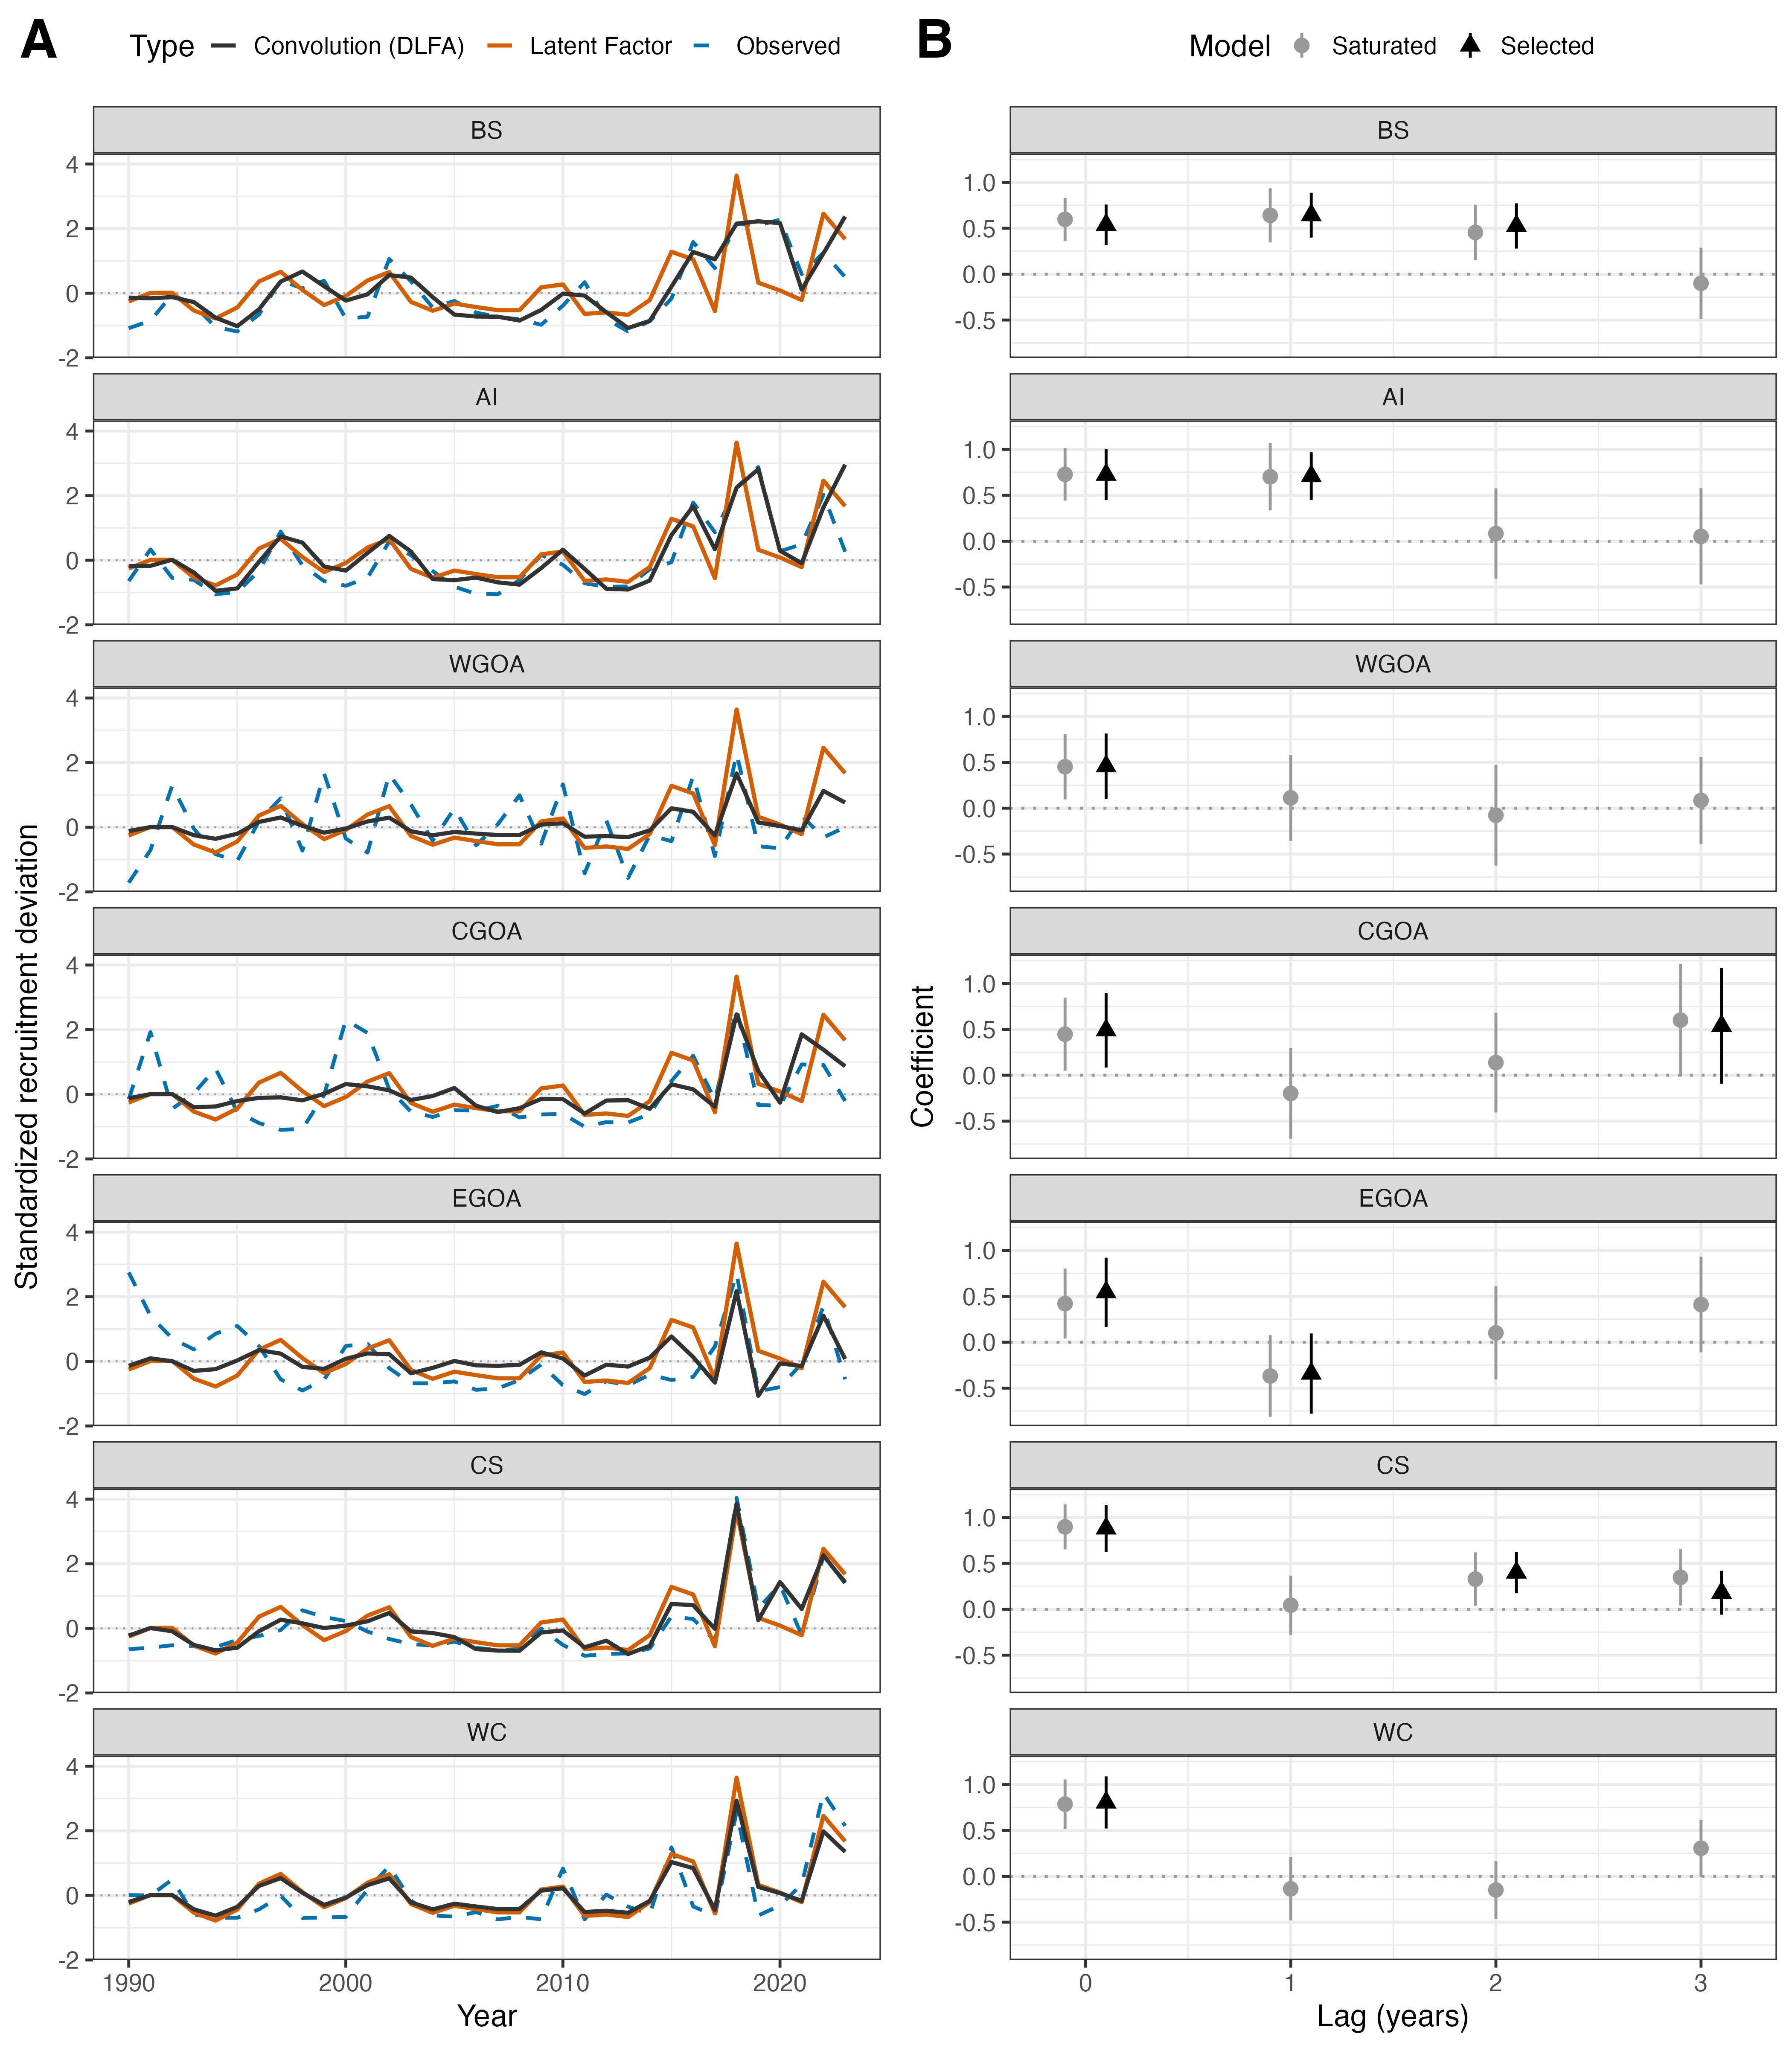
\includegraphics[width=1\textwidth]{figs/ts_lag_comp.png}
    \caption{
    Estimated recruitment deviations (panel A) or lagged responses
    (panel B) by region (rows, ordered from Northwest to Southeast). For
    recruitment deviations, we show the recruitment deviations (y-axis)
    by year (x-axis) including stock assessment model-output
    ("observations") (blue dashed line), the estimated latent factor
    (orange line), or the factor after its convolution using a
    distributed lag (black line). Results for panel A only show the
    selected model. For the lagged responses, we show the estimated
    response (y-axis) by lag (x-axis, where a lag-0 represents a
    synchronous response mimicking a traditional DFA) for either the
    full ("saturated") model (grey) or the selected model using the
    marginal Akaike Information Criterion (black), where whiskers are
    approximate 95\% confidence intervals.
    }
    \label{fig:ts_lag_comp}
\end{figure}

\clearpage

\begin{figure}[htb]
    \centering
    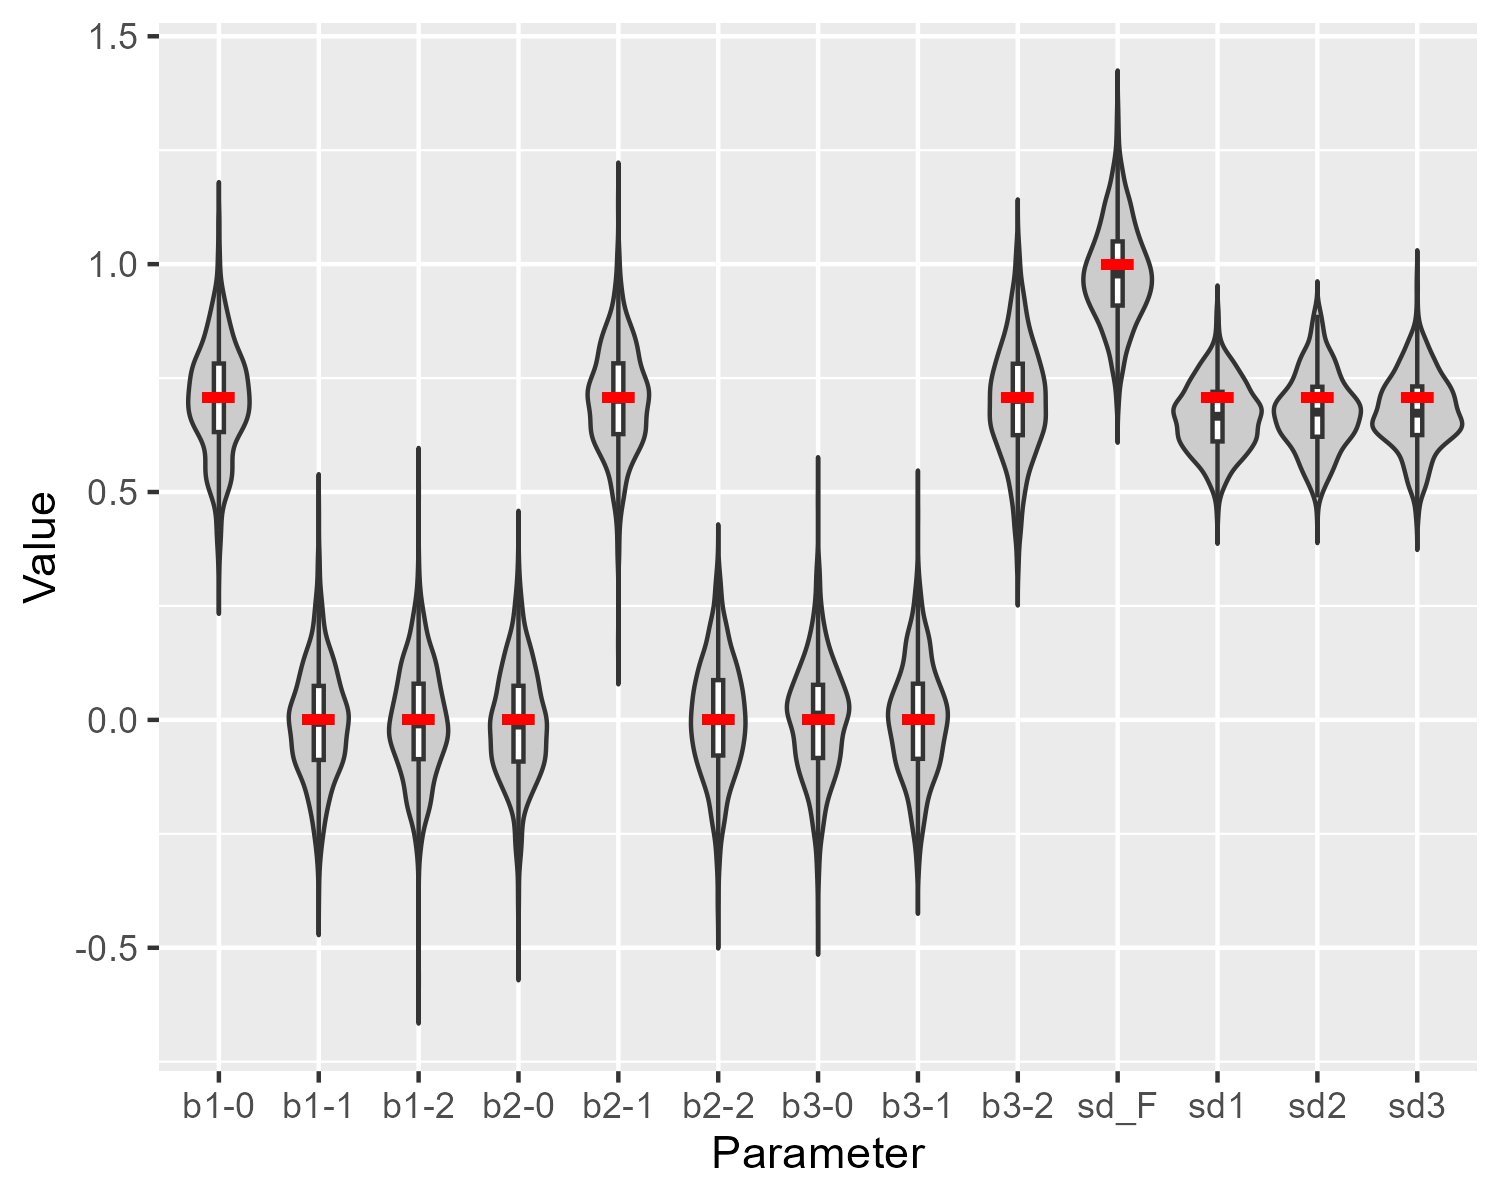
\includegraphics[width=1\textwidth]{simulation/simulation.png}
    \caption{
    Estimation performance in a self-test simulation experiment, showing
    the distribution of estimated factor loadings across 500 simulation
    replicates (y-axis) for parameters (x-axis) representing
    synchronous, lag-1, and lag-2 responses to a single simulated factor
    (e.g., \texttt{b1-0} for loading of area-1 at lag-0), as well as the
    estimated standard deviation for residual errors for each region
    (e.g., \textttt{sd1} is the standard deviation for area-1) relative
    to the true simulated value (red line).
    }
    \label{fig:simulation}
\end{figure}

\clearpage

\end{document}
